% ---------------------------------------------------------------------------
% Author guideline and sample document for EG publication using LaTeX2e input
% D.Fellner, v1.13, Jul 31, 2008

\documentclass{egpubl}
\usepackage{eg2017}

% --- for  Annual CONFERENCE
% \ConferenceSubmission   % uncomment for Conference submission
% \ConferencePaper        % uncomment for (final) Conference Paper
\STAR                   % uncomment for STAR contribution
% \Tutorial               % uncomment for Tutorial contribution
% \ShortPresentation      % uncomment for (final) Short Conference Presentation
% \Areas                  % uncomment for Areas contribution
% \MedicalPrize           % uncomment for Medical Prize contribution
% \Education              % uncomment for Education contribution
%
% --- for  CGF Journal
% \JournalSubmission    % uncomment for submission to Computer Graphics Forum
% \JournalPaper         % uncomment for final version of Journal Paper
%
% --- for  EG Workshop Proceedings
% \WsSubmission    % uncomment for submission to EG Workshop
% \WsPaper         % uncomment for final version of EG Workshop contribution
%
 \electronicVersion % can be used both for the printed and electronic version

% !! *please* don't change anything above
% !! unless you REALLY know what you are doing
% ------------------------------------------------------------------------

% for including postscript figures
% mind: package option 'draft' will replace PS figure by a filname within a frame
\ifpdf \usepackage[pdftex]{graphicx} \pdfcompresslevel=9
\else \usepackage[dvips]{graphicx} \fi

\PrintedOrElectronic

% prepare for electronic version of your document
\usepackage{t1enc,dfadobe}

\usepackage{egweblnk}
\usepackage{cite}

%%%%%%%%%%%%%%%%%%%%%%%%%%%%%%%%%%%%%%%%%%%%%%%%%%%%%%%%%%%%%%%%
\usepackage{graphicx}	% A package for graphics use (see figures)

%% subfigure and subcaption
\usepackage{caption}
\usepackage{subcaption}
%% bookmark
\usepackage{hyperref}
\usepackage{bookmark,hyperref}
%% url
\usepackage{url}

%% Math Packages %%%%%%%%%%%%%%%%%%%%%%%%%%%%%%%%%%%%%%%%%%%%
\usepackage{amssymb}
\usepackage{amsmath}
\usepackage{amsfonts}

% other packages
\usepackage{braket}

%for including pdf
\usepackage{pdfpages}
\graphicspath{{figures/}{images/}}
%%%%%%%%%%%%%%%%%%%%%%%%%%%%%%%%%%%%%%%%%%%%%%%%%%%%%%%%%%%%%%%%

% For backwards compatibility to old LaTeX type font selection.
% Uncomment if your document adheres to LaTeX2e recommendations.
% \let\rm=\rmfamily    \let\sf=\sffamily    \let\tt=\ttfamily
% \let\it=\itshape     \let\sl=\slshape     \let\sc=\scshape
% \let\bf=\bfseries

% end of prologue

% ---------------------------------------------------------------------
% EG author guidelines plus sample file for EG publication using LaTeX2e input
% D.Fellner, v1.17, Sep 23, 2010


\title%[EG \LaTeX\ Author Guidelines]%
{
%\LaTeX\ Author Guidelines for EUROGRAPHICS Proceedings Manuscripts
A Survey on Automated Transfer Function Design and Optimization for Volume Visualization}

% for anonymous conference submission please enter your SUBMISSION ID
% instead of the author's name (and leave the affiliation blank) !!
%\author%[D. Fellner \& S. Behnke]
%{
%%	D.\,W. Fellner\thanks{Chairman Eurographics Publications Board}$^{1,2}$
%%	and S. Behnke$^{2}$
%%	%        S. Spencer$^2$\thanks{Chairman Siggraph Publications Board}
%%	\\
%%	% For Computer Graphics Forum: Please use the abbreviation of your first name.
%%	$^1$TU Darmstadt \& Fraunhofer IGD, Germany\\
%%	$^2$Institut f{\"u}r ComputerGraphik \& Wissensvisualisierung, TU Graz, Austria
%%	%        $^2$ Another Department to illustrate the use in papers from authors
%%	%             with different affiliations
%}
\author[S. Luo \& J. Dingliana]
{Shengzhou Luo
and
John Dingliana
\\
Graphics Vision and Visualisation group (GV2), Trinity College Dublin
}
% ------------------------------------------------------------------------

% if the Editors-in-Chief have given you the data, you may uncomment
% the following five lines and insert it here
%
% \volume{27}   % the volume in which the issue will be published;
% \issue{1}     % the issue number of the publication
% \pStartPage{1}      % set starting page


%-------------------------------------------------------------------------
\begin{document}
	
%	\teaser{
%		
\includegraphics[width=\linewidth]{eg_new}
%		\centering
%		\caption{New EG Logo}
%		\label{fig:teaser}
%	}
	
\maketitle

%\begin{abstract}
%	The ABSTRACT is to be in fully-justified italicized text, 
%	between two horizontal lines,
%	in one-column format, 
%	below the author and affiliation information. 
%	Use the word ``Abstract'' as the title, in 9-point Times, boldface type, 
%	left-aligned to the text, initially capitalized. 
%	The abstract is to be in 9-point, single-spaced type.
%	The abstract may be up to 3 inches (7.62 cm) long. \\
%	Leave one blank line after the abstract, 
%	then add the subject categories according to the ACM Classification Index 
%	(see http://www.acm.org/class/1998/).
%	
%	\begin{classification} % according to http://www.acm.org/class/1998/
%		\CCScat{Computer Graphics}{I.3.3}{Picture/Image Generation}{Line and curve generation}
%	\end{classification}
%	
%\end{abstract}

%-------------------------------------------------------------------------
\section{Introduction}
Volume data are 3D entities with information inside them, but the data might not consist of surfaces and edges.
%, or might be too voluminous to be represented geometrically.
%The goal of volume visualization is to gain insightful depictions of volume data.
Because of the lack of explicit geometric information, %and limited semantics, 
it is a major challenge to provide clear visualizations of the structures contained in a volume data set.
Volume data may be rendered directly by mapping scalar values to visual properties (e.g. opacity and color), or an intermediate geometric representation may be extracted using techniques like Marching Cubes \cite{lorensen_marching_1987} and then rendered as geometric surfaces. The mapping, which assigns visual properties to volume data, is called a transfer function.

Motivated by scientific visualization and medical imaging, where volume data is often acquired by devices such as CT and MRI scanners, or numerical simulation of natural phenomena, researchers have developed a wide variety of techniques to improve the performance and enhance the perception of volume visualization \cite{corcoran_enhancing_2013}.

%% ================================================================
\section{Transfer Functions}
Transfer function specification is an essential part in volume visualization.
%In terms of dimensionality, transfer functions are divided into two categories, one-dimensional (1D) and multidimensional.
A simple one-dimensional transfer function is a mapping from scalar values to RGB and alpha values.
The resulting visualization largely depends on how well the transfer function captures features of interest \cite{kniss_multidimensional_2002}.
%Due to the complex nature of volumetric data sets, abstraction techniques is often used in order to provide better understanding of the data sets.
However, it is non-trivial to obtain an effective transfer function. The specification is often achieved by a trial-and-error process, which involves a significant amount of tweaking of color and opacity. Figure~\ref{fig:multiple_glk_transfunction} shows how slight changes in the transfer function lead to significant changes in the resulting images. The adjustment of transfer functions is unintuitive and often difficult.

In practice, major factors that have a great influence on transfer function setting are: partial volume effect \footnote{During the acquisition of data, the finite resolution causes contributions of different materials combined into the value of a single voxel. This is generally referred to as the partial volume effect, which results in blurred boundaries and hampers the detection of small or thin structures. \cite{serlie_classifying_2007}}, non-uniform distribution of materials and noise \cite{serlie_computed_2003}.
Among these, two challenging problems that need to be tackled could be elaborated as follows: firstly, for volume data sets, e.g. those obtained by MRI and CT, different tissues are represented in similar or even overlapping ranges of scalar values; secondly, interesting interior structures are often partly or completely occluded by surrounding tissue.
%This is common in visualizing interior structures. 
%Consequently, feature detection and understanding volume data become a big challenge.

\begin{figure}
	\centering
	\begin{minipage}{0.4\textwidth}
		\centering
		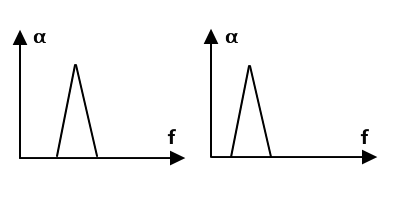
\includegraphics[width=1\linewidth]{images/glk_transfunction_tf.png}
		\subcaption{Two transfer functions (TF)}
		%                \label{fig:glk_transfunction_tf}
	\end{minipage}
	\begin{minipage}{0.2\textwidth}
		\centering
		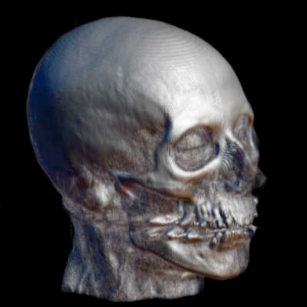
\includegraphics[width=1\linewidth]{images/glk_transfunction_1.png}
		\subcaption{The result from the TF on the left in (a)}
		%                \label{fig:glk_transfunction_1}
	\end{minipage}~
%add desired spacing between images, e. g. ~, \quad, \qquad etc.
%(or a blank line to force the subfigure onto a new line)        
	\begin{minipage}{0.2\textwidth}
		\centering
		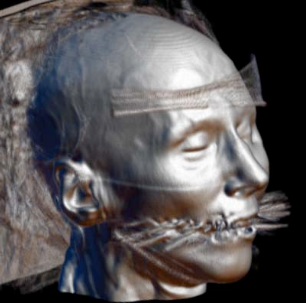
\includegraphics[width=1\linewidth]{images/glk_transfunction_2.png}
		\subcaption{The result from the TF on the right in (a)}
		%                \label{fig:glk_transfunction_2}
	\end{minipage}    
	\caption{Slight changes in the transfer function causes significant difference in the resulting images \cite{kindlmann_transfer_2002}}
	\label{fig:multiple_glk_transfunction}
\end{figure}

These problems are handled by transfer functions, which have played a crucial role in volume visualization.
%Transfer functions have played a crucial role in volume visualization.
Good transfer functions reveal important structures in the data without obscuring them with less important regions.
%Traditional one-dimensional transfer function approaches, which assign optical properties only based on scalar value, are inadequate to extract inner structures of interest from volume data.
%Various strategies have been proposed to simplify transfer function specification \cite{pfister_transfer_2001}.
The design of transfer functions to generate informative visualizations has been a significant challenge addressed by a number of researchers \cite{pfister_transfer_2001}.
Various strategies have been proposed for transfer function design \cite{hadwiger_real-time_2006}.
%Data-centric strategies examine the properties of volume data sets.
%However, certain features are difficult to be extracted and visualized with 1D transfer functions, e.g. CT and MRI data sets which contain complex boundaries between multiple materials.
%Overlapping intensity intervals corresponding to different materials make boundary separation difficult.
However, features with overlapping intensity intervals are difficult to extract and visualize with 1D transfer functions.
When one intensity value or interval is associated with multiple boundaries, a 1D transfer function is unable to render them in isolation \cite{kniss_multidimensional_2002}.
%Overlapping intensity intervals corresponding to different materials make boundary detection difficult.
%However, certain features of interest in volume data are difficult to extract and visualize with 1D transfer functions. For instance, many medical data sets created from CT or MRI scans contain a complex combination of boundaries between multiple materials. This situation is problematic for 1D transfer functions because of the potential for overlap between the data value intervals spanned by the different boundaries. When one data value or data range is associated with multiple boundaries, a 1D transfer function is unable to render them in isolation \cite{kniss_multidimensional_2002}.

Classical approaches to this problem try to detect boundary information between tissues by introducing derived attributes such as first and second-order derivatives to isolate materials \cite{kindlmann_semi-automatic_1998} \cite{kniss_multidimensional_2002}. In this case, the transfer functions are extended to multidimensional feature spaces. 
The introduction of multidimensional transfer functions alleviates the material separation problem.
Instead of classifying a voxel based on a single scalar value, multidimensional transfer functions allow a voxel to be classified based on a combination of values.
Multidimensional transfer functions are very effective means to extract materials and their boundaries for both scalar and multivariate data.
%Multidimensional transfer functions are discussed in more detail in the next subsection.

In addition, various user interfaces were proposed to simplify the design of multidimensional transfer functions \cite{tzeng_novel_2003} \cite{tzeng_cluster-space_2004}.
However, the parameter spaces of multidimensional transfer functions are more complex (compared to 1D transfer functions) and thus introduce problems such as requirement for large amount of user interaction, missing precision or the interaction being complex and unintuitive \cite{arens_survey_2010}.
%As a result, the interaction of transfer functions becomes more complex and unintuitive.

Another strategy is based on the selection of rendered images. This strategy lets the user select one or more favorite images to guide the further search of transfer functions \cite{marks_design_1997} \cite{wu_interactive_2007}. More recent approaches introduced visibility \cite{correa_visibility-driven_2009} \cite{correa_visibility_2011} or measures derived from information theory \cite{haidacher_information-based_2008} \cite{bruckner_isosurface_2010} \cite{ruiz_automatic_2011} \cite{bramon_information_2013}. Zhou et al. studied the combination of 2D transfer functions with occlusion and size-based transfer functions \cite{zhou_transfer_2012}.

Bruckner and Gr{\"o}ller introduced the concept of style transfer functions \cite{bruckner_style_2007}, which aim to produce more comprehensible images by using transfer functions that map input values to different non-photorealistic rendering styles.

Despite the advances of these methods, transfer function design for volume rendering is still an open research problem.
The creation of transfer functions needs to be simplified and the functionality of transfer functions needs to be extended in order to realize the full potential of volume rendering. For instance, more sophisticated transfer functions are required in medical imaging, in order to address various domain specific visualization problems \cite{lindholm_spatial_2010}.

Moreover, transfer function specification in general is an unintuitive or even monotonous task for average users, because it usually involves an iterative process of trial and error.
For instance, there are skin and fat tissues around the brain, and their intensities lie in the same range as the brain. If we want to visualize the brain by setting the scalar value range of the brain to opaque, the surrounding skin and fat tissue will also become opaque. Then the brain will be occluded by the surrounding soft tissues which make it difficult to explore the brain structure.
Common approaches to this problem are introducing explicit segmentation of structures of interest before the volume rendering process \cite{rezk-salama_opacity_2006}. In fact, the process of applying the transfer function could be interpreted as a segmentation problem.
%-------------------------------------------------------------------------
%-------------------------------------------------------------------------

\subsection{1D Transfer Functions}

\begin{table}
	\centering
	%\begin{minipage}{.5\textwidth}
	\normalsize
	\begin{tabular}{llll}
		\hline
		air & fat & soft tissue & bone (cancellous/dense)\\
		\hline
		-1000 & -100 to -50 & +100 to +300 & +700 to +3000\\
		\hline
	\end{tabular}
	\caption{Hounsfield units of some typical substances \cite{feeman_mathematics_2009}}
	\label{table:Hounsfield_unit}
	%\end{minipage}
\end{table}

\begin{figure}
	\centering
	
	\begin{subfigure}{.2\textwidth}
		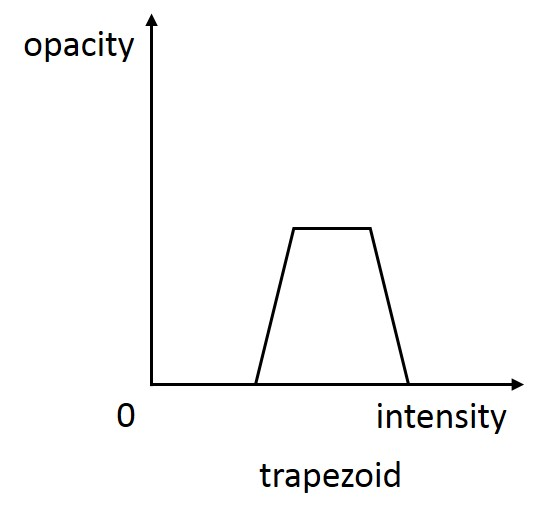
\includegraphics[width=1\textwidth]{konig_mastering_2000-zhou_automatic_2009_a.jpg}
	\end{subfigure}
	\begin{subfigure}{.2\textwidth}
		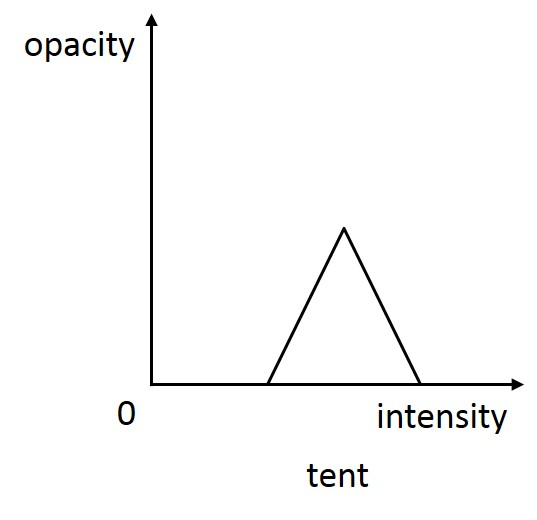
\includegraphics[width=1\textwidth]{konig_mastering_2000-zhou_automatic_2009_b.jpg}
	\end{subfigure}
	\begin{subfigure}{.2\textwidth}
		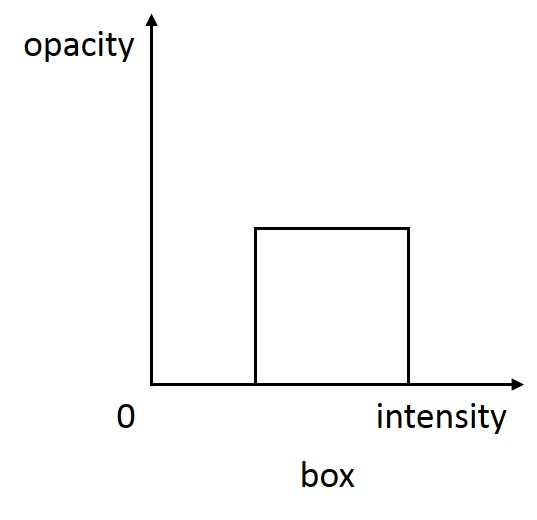
\includegraphics[width=1\textwidth]{konig_mastering_2000-zhou_automatic_2009_c.jpg}
	\end{subfigure}
	\begin{subfigure}{.2\textwidth}
		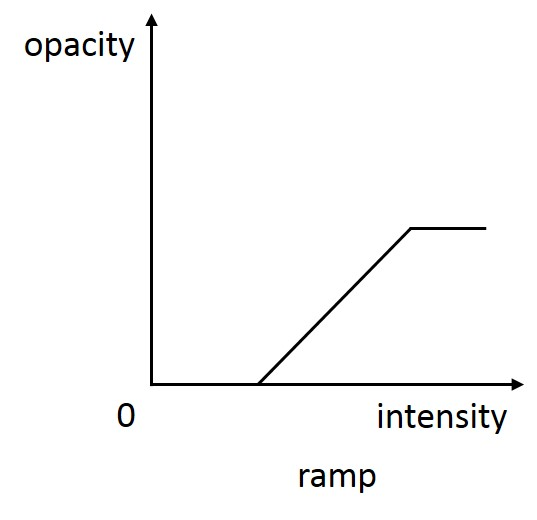
\includegraphics[width=1\textwidth]{konig_mastering_2000-zhou_automatic_2009_d.jpg}
	\end{subfigure}
	\caption{Typical transfer function shapes \cite{konig_mastering_2000}}
	\label{fig:konig_mastering_2000}
	\begin{subfigure}{.4\textwidth}
		\centering
		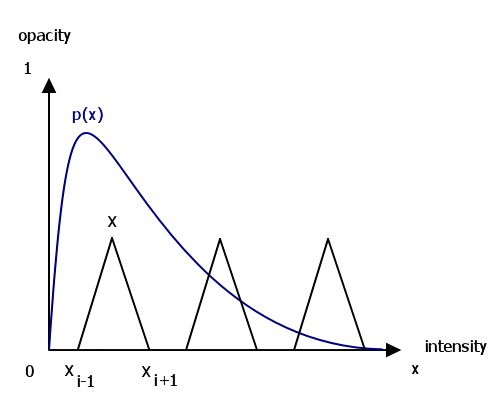
\includegraphics[width=1\textwidth]{drawing_distribution.png}
	\end{subfigure}
	\caption{A transfer function with tent-like shapes}
	\label{fig:drawing_distribution}
\end{figure}

In the specification of a 1D (intensity-based) transfer function, the user essentially assigns a color and/or opacity to a certain point in the histogram of scalar values in the data set. In practice, the user would be presented with an interface that allows them to set up several control points which corresponds to a certain kind of material or structure. The user then defines a mapping from each control point to some visual property (e.g. color) resulting in voxels of the corresponding intensity to be rendered in that color.
Figure~\ref{fig:konig_mastering_2000} displays four typical shapes used in transfer function design.
%All the four shapes can reveal structures in volume data sets.
If a volume data set contains complex structures, tent-like shapes are desirable in revealing isosurfaces of structures and seeing through inner structures. Otherwise, the ramp shape and other shapes can also reveal structures effectively.% \cite{zhou_automatic_2009}

In order to design transfer functions effectively, it is commonly required that users have prior knowledge about which intensity ranges are relevant or which regions should be emphasized in the data. This is especially the case in medical visualization. For instance, in computed tomography (CT) data the intensity ranges are determined by the Hounsfield scale (Table~\ref{table:Hounsfield_unit}). The user may expect the constituent's intensity of CT data to follow the Hounsfield scale and thus set up control points accordingly.


Another consideration is that interior structures are likely to comprise far fewer voxels and are often occluded by the surrounding material.
Consider the transfer function in Figure~\ref{fig:drawing_distribution}. The user finds three intensity intervals of interest and then sets up three sets of control points in order to visualize these intensity intervals. The opacity of the three peak control points are assigned equally as they are equally important.
However, if the distribution of voxels follows $ p(x) $ (the blue curve), the voxels of the leftmost intensity intervals may completely occlude voxels of the other two intensity intervals in the resulting image.


\subsection{Multidimensional Transfer Functions}
Multidimensional transfer functions \cite{kniss_interactive_2001}, which are mappings from intensity and other variables, such as first and second derivatives to color and opacity, have demonstrated their effectiveness in distinguishing boundaries between materials in volume data.



In volume data, boundaries are regions between areas of relatively homogeneous material. It is difficult to detect boundaries because different materials often consist of overlapping intensity intervals. To address this problem, multidimensional transfer functions used derived attributes such as gradient magnitudes and second derivatives along with scalar values, in order to detect transitions between relatively homogeneous areas \cite{kindlmann_semi-automatic_1998} \cite{kindlmann_transfer_2002}.


In this case, the transfer functions are extended to multidimensional feature spaces.
For higher-dimensional transfer functions, the generation of transfer functions could be memory intensive and costly to compute, and the interaction of transfer functions are more complex and unintuitive as the dimensionality becomes higher. 

Therefore, two-dimensional (2D) histograms are often used in multidimensional transfer functions \cite{maciejewski_structuring_2009}. An example is a 2D histogram with axes representing a subset of the feature space (e.g. scalar value vs gradient magnitude), with each entry in the 2D histogram being the number of voxels for a given feature space pair.
Even in the case of two-dimensional transfer functions, a considerable amount of user interaction is required in order to come up with meaningful results \cite{arens_survey_2010}.



As one of the most common representations of voxel distributions, histograms are used in transfer function design to assign visual properties to voxels \cite{pfister_transfer_2001}. Bajaj et al. \cite{bajaj_contour_1997} introduced the contour spectrum to determine voxels corresponding to important isosurfaces in the volume. To overcome the difficulty of using one-dimensional transfer functions (solely based on scalar values stored in the voxels) to extract inner structures of interest from the volume data, Levoy \cite{levoy_display_1988} proposed the use of gradient magnitude to emphasize strong boundaries between different tissues.

The introduction of gradient magnitude as a data metric aims to detect voxels that are of large deviation compared with other voxels by approximating gradient magnitude at each sample point in the volume, because the exact distribution of data is unknown due to information lost in the discrete sampling process.
Kindlmann and Durkin \cite{kindlmann_semi-automatic_1998} extended Levoy's work \cite{levoy_display_1988} by introducing a higher dimensional transfer function domain based on gradient magnitudes and second derivatives. To emphasize different structures, Kniss et al. \cite{kniss_interactive_2001} presented a technique for interactively manipulating 2D histograms of gradient magnitudes and data values. In their work, material boundaries appear as arcs in the 2D histogram and can be selected with interactive widgets \cite{kniss_multidimensional_2002}.
Kniss et al. \cite{kniss_gaussian_2003} presented Gaussian transfer functions, which are suitable for the classification of narrow features in multidimensional domains.

Kindlmann et al. \cite{kindlmann_curvature-based_2003} proposed curvature-based transfer function to enhance the expressive and informative power of volume rendering. In their approach, volume data is rendered with contours to exhibit constant thickness in image space.

{\v S}ereda et al. \cite{sereda_visualization_2006} proposed LH histograms for improving the identification and selection of boundaries in 2D intensity-gradient transfer functions. Subsequently, {\v S}ereda et al. \cite{sereda_automating_2006} presented a clustering method based on the LH histograms for semi-automatic transfer function design.

Haidacher et al. \cite{haidacher_volume_2010} described the statistical transfer function space, which is based on statistical properties such as mean and standard deviation of the data values (e.g. intensity and gradient magnitude for 2D transfer functions) in the neighborhood of each voxel. This approach can reduce the influence of noise and enhance visual appearance in volume rendering.

Wang et al. \cite{wang_automating_2012} described a clustering approach on 2D density plots for automatic transfer function design. Their approach allows the user to interactively explore the pre-computed clusters in the feature space and merge or remove uninterested features to improve visualization quality.
Ip et al. \cite{ip_hierarchical_2012} described a multilevel segmentation technique that mimics user exploration behaviors by recursively segmenting intensity-gradient histograms.

There are other multidimensional transfer function approaches, such as spatialized gradient-based transfer functions \cite{roettger_spatialized_2005}, distance-based transfer functions \cite{tappenbeck_distance-based_2006}, size-based transfer function \cite{correa_size-based_2008}, texture-based transfer functions \cite{caban_texture-based_2008} \cite{alper_selver_exploring_2015}.
% and curvature based transfer functions \cite{kindlmann_curvature-based_2003}.

In addition, parallel coordinates and dimensionality reduction algorithms (e.g. principal component analysis) have been employed to support the design of transfer functions in multidimensional parameter spaces \cite{zhao_multi-dimensional_2010} \cite{guo_multi-dimensional_2011} \cite{kim_dimensionality_2010}.

\section{Entropy, Visibility and Saliency in Volume Visualization}
Transfer function specification is an unintuitive task often achieved using subjective manual input. For generalizable solutions, it is desirable to have objective feedback regarding the clarity of features in volume visualization.

\subsection{Entropy of Volume Data}
In computer graphics, information-theoretic measures, such as entropy and mutual information, have been applied to solve multiple problems in areas such as view selection \cite{bordoloi_view_2005} 
%\cite{takahashi_feature-driven_2005}
\cite{bramon_information-theoretic_2013}, flow visualization \cite{xu_information-theoretic_2010}, multi-modal visualization \cite{haidacher_information-based_2008} \cite{bramon_information_2013} and transfer function design \cite{bruckner_isosurface_2010} \cite{ip_hierarchical_2012}.
Information theory provides a theoretic framework to measure the information content (or uncertainty) of a random variable represented as a distribution \cite{wang_information_2011}.
Consider a discrete random variable X which has a set of possible values $\{a_{0},a_{1},...,a_{n-1} \}$ with probabilities of occurrence $\{ p_{0},p_{1},...,p_{n-1} \}$, we can measure the uncertainty of the outcome with the entropy H(X), which is defined by
\[  H(X)=-\sum_{x \in X} p(x) \log p(x) 
%\addtag
\]
where the summation is over the corresponding alphabet and the convention $ 0\log 0=0 $ is taken% \cite{sbert_information_2011}
.
The term $ -\log p(x) $ represents the information content associated with the result x.
If the entire volume data set is treated as a random variable, $ I(a_{x})=-\log p(x) $ represents the information content of a voxel $ a_{x} $ with intensity x, and the entropy gives us the average amount of information of a volume data.
The probability p(x) is defined by
$ p(x)=\frac{n_{x}}{n} $, where $ n_{x} $ is the number of voxels with intensity x and n is the total number of voxels in the volume data.


Bordoloi and Shen \cite{bordoloi_view_2005} described a noteworthiness factor to denote the significance of the voxel to the visualization.
The noteworthiness should be high for the voxels which are desired to be seen, and vice versa. The noteworthiness of voxel $ j $ is defined as
$ W_{j}=\alpha_{j}I_{j}=-\alpha_{j}log f_{j} $
, where $ \alpha_{j} $ is the opacity of voxel $ j $ looked up from the transfer function, $ I_{j} $ is the information carried by voxel $ j $, which can be derived from the frequency of its histogram bin $ f_{j} $. $ -log f_{j} $ represents the amount of information associated with voxel $ j $.


%-------------------------------------------------------------------------	
\subsection{Visibility and Saliency Measures}

Visibility measures the impact of individual voxels on the image generated by a volumetric object and visibility distribution can be utilized as a measure on the quality of transfer functions as users explore the transfer function space. Visibility has been studied to measure the quality of a given viewpoint \cite{bordoloi_view_2005} \cite{viola_importance-driven_2004} and to enhance the rendering process with cutaway views.
%Correa and Ma \cite{correa_visibility_2011} introduced visibility histogram, which describes the accumulated visibility of each intensity value in the transfer function.
%Wang et al. \cite{wang_efficient_2011} extended the idea of the visibility histogram to feature visibility and introduced an interaction scheme where the opacity of each feature was generated automatically based on user-defined visibility values. Visibility distribution is also used in automating color mapping \cite{cai_automatic_2013} and 2D transfer functions \cite{qin_voxel_2015}.

Although many approaches in volume visualization attribute the visibility of a feature to its transparency and level of occlusion by other features, it is important to note that the ability of a viewer to perceive features can be strongly affected by how it stands out against others in its neighborhood. Thus an understanding of salient regions in images \cite{zhao_learning_2013} can be useful for improving visualizations.

Inspired by mechanisms of the human visual system, several computational models of visual saliency for modeling human attention have been developed \cite{harel_graph-based_2006}.
Itti et al. \cite{itti_model_1998} developed a computational model of visual attention based on the center-surround operators in an image. This center-surround mechanism has the intuitive appeal of being able to identify regions that are different from their surrounding context.

Lee et al. \cite{lee_mesh_2005} presented mesh saliency, which is defined in a scale-dependent manner using a center-surround operator on Gaussian-weighted mean curvatures.
%They observed that their approach was able to capture the most visually interesting regions on a mesh.
In the scope of volume visualization, Kim and Varshney \cite{kim_saliency-guided_2006} introduced the use of center-surround operators to compute saliency fields of volume data sets.
%In their user study, they found that their approach was better at eliciting viewer attention than the traditional Gaussian regional enhancement approaches.

Based on perceptual principles, Chan et al. \cite{chan_perception-based_2009} introduced several image quality measures to enhance the perceived quality of semitransparent features.
J{\"a}nicke and Chen \cite{janicke_salience-based_2010} described a quality metric for analyzing the saliency of visualization images and demonstrated its usefulness with examples from information visualization, volume visualization and flow visualization.

Shen et al. \cite{shen_save:_2014} proposed the use of saliency to assist volume exploration. They described a method for inferring interaction position in volume visualization, in order to help users pick focused features conveniently.
Shen et al. \cite{shen_spatiotemporal_2015} described spatiotemporal volume saliency, which extended the saliency field \cite{kim_saliency-guided_2006} to time-varying volume data. Luo and Dingliana \cite{luo_visibility-weighted_2015} proposed a visibility-weighted saliency metric that combines both aspects of visibility and saliency.

\subsection{Visibility Histograms and Visibility-Driven Transfer Functions}
Visibility has been studied in measuring viewpoint quality \cite{bordoloi_view_2005} and enhancing ghost and cutaway views \cite{viola_importance-driven_2004} in volume visualization.

In traditional transfer function design, the visibility of structures revealed in volume rendering is a consequence of adjusting transfer function parameters, rather than a design parameter \cite{preim_visual_2013}.
Correa and Ma \cite{correa_visibility-driven_2009} introduced visibility histograms to guide transfer function design for both manual and automatic adjustment.
Visibility histograms (Figure~\ref{fig:correa_visibility-driven_2009}), which summarize the distribution of visibility of voxels from a given viewpoint, are powerful feedback mechanisms of volume visualization \cite{emsenhuber_visibility_2008}.
Visibility histograms encode the information required to measure the efficacy of transfer functions and are advantageous in guiding and automating the manipulation of transfer functions.

\begin{figure}
	\centering
	\begin{minipage}{.24\textwidth}
		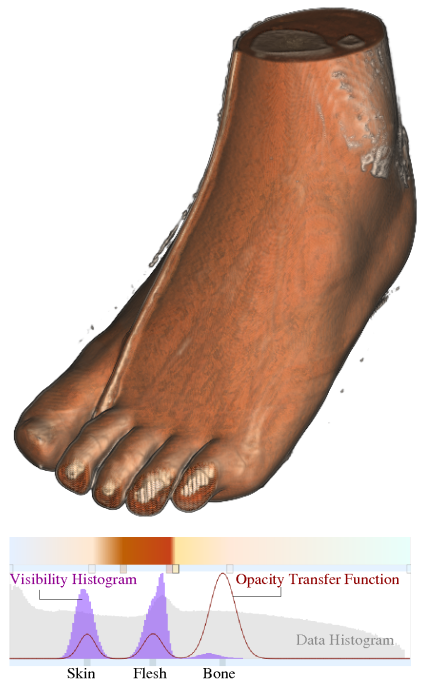
\includegraphics[width=1\linewidth]{images/correa_visibility-driven_2009_a}
		\subcaption{A user-defined opacity transfer function and the initial visibility histogram}
	\end{minipage}~
	\begin{minipage}{.24\textwidth}
		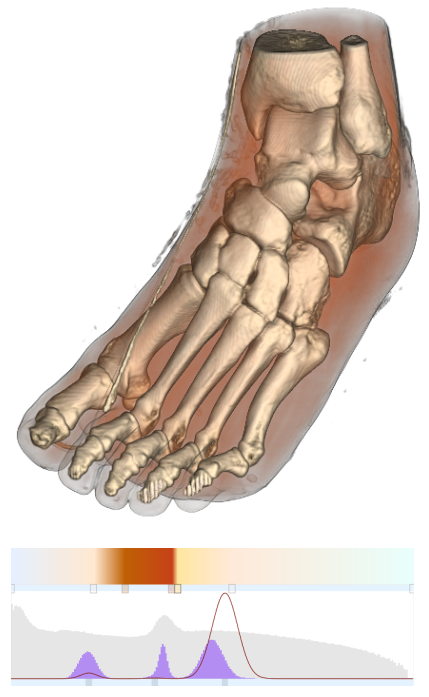
\includegraphics[width=1\linewidth]{images/correa_visibility-driven_2009_b}
		\subcaption{Here the visibility histogram has been modified to match the user-defined opacity transfer function.}
	\end{minipage}
	\caption{Visibility histograms \cite{correa_visibility-driven_2009}}
	\label{fig:correa_visibility-driven_2009}
\end{figure}
 
Wang et al. \cite{wang_efficient_2011} extended the previous work on visibility histograms and proposed a feature visibility metric,
in order to measure the influence of each feature to the volume rendered image. As shown in Figure~\ref{fig:wang_efficient_2011}, their approach allows the user to directly specify the desired visibility for the features of interest, and subsequently the opacity transfer function is optimized using an active set algorithm \cite{polyak_conjugate_1969}.

\begin{figure}
	\centering
	\begin{minipage}{.24\textwidth}
		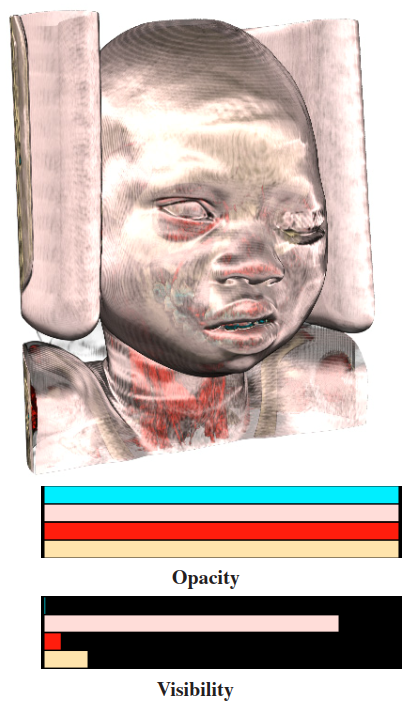
\includegraphics[width=1\linewidth]{images/wang_efficient_2011_a}
		\subcaption{Feature opacities are equal}
	\end{minipage}~
	\begin{minipage}{.24\textwidth}
		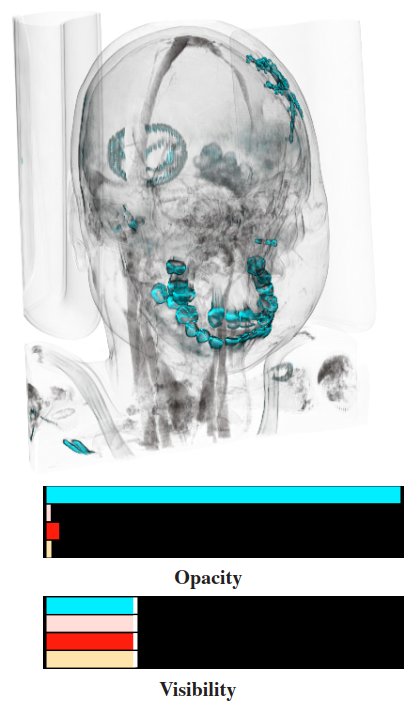
\includegraphics[width=1\linewidth]{images/wang_efficient_2011_b}
		\subcaption{Feature visibilities are equal}
	\end{minipage}
	\caption{Opacities and feature visibilities of 4 features highlighted in different colors \cite{wang_efficient_2011}}
	\label{fig:wang_efficient_2011}
\end{figure}

Ruiz et al. \cite{ruiz_automatic_2011} proposed an information-theoretic framework which obtains opacity transfer functions by minimizing the Kullback-Leibler divergence between the observed visibility distribution and a target distribution provided by the user. Later, Bramon et al. \cite{bramon_information_2013} extended this approach to visualize multimodal volume data.

Cai et al. \cite{cai_automatic_2013} described a method to derive opacity transfer functions by minimizing the Jensen-Shannon divergence between the observed visibility distribution and a user-defined target distribution. The target distribution can be defined using Gaussian function weighting.



In addition, various methods were proposed regarding the use of visibility for enhancing different aspects of volume visualization.
Marchesin et al. \cite{marchesin_per-pixel_2010} introduced a volume rendering technique that manipulates the voxel opacity values in a view-dependent way, in order to enhance visibility of internal structures in the volume data set.
Bronstad et al. \cite{bronstad_visibility_2012} described local opacity transfer functions with feature detection along the ray profile implemented on the GPU. In their approach, visibility histograms are employed to access the performance of the feature detection algorithm.

Jung et al. \cite{jung_dual-modal_2012} presented a dual-modal visualization method, which uses visibility metrics to provide visual feedback regarding the occlusion caused by the volume data in one modal on the other modal.
Jung et al. \cite{jung_visibility-driven_2013} extended visibility histograms to multimodal volume visualization.
They demonstrated the use of visibility histograms together with region of interest segmentation was effective in visualizing PET-CT volume data sets.

Instead of computing the visibility of all voxels, Zheng et al. \cite{zheng_visibility_2013} employed local visibility histograms to ensure both the features of interest and contextual information are visible in multimodal volume visualization.
Schlegel and Pajarola \cite{schlegel_visibility-difference_2013} proposed a visibility-difference entropy metric. They presented an automated approach using this metric for generating a set of transfer function candidates with high ratings and are strongly distinct in what they reveal.

Qin et al. \cite{qin_voxel_2015} presented the voxel visibility model as a quality metric for transfer function design.
The voxel visibility model is a mapping function from data attributes of voxels to their visibility attributes. Instead of specifying transfer functions, this approach allows users to directly adjust the visibility of each voxel, and then the corresponding opacity transfer functions can be obtained by minimizing the distance between the desired voxel visibility distriubtion and the actual voxel visibility distribution.

%-------------------------------------------------------------------------
\subsection{Visibility-Based Sketching and Picking}

The visibility of a sample refers to the alpha contribution of a sample to the final image, taking into account also the degree to which it is occluded by other samples in the view.
%This visibility can be computed as the difference between the accumulated alpha of a sample and the accumulated alpha of the previous sample along a ray in volume ray-casting.
%Correa et al. presented the general notion of visibility histograms \cite{correa_visibility_2011} which represent the distribution of visibility over intensity ranges in a volume rendering image.

Guo et al. \cite{guo_wysiwyg_2011} proposed a sketch-based manipulation technique for volume visualization based on clustering of depth, visibility, alpha and intensity. Subsequently, they described another sketch-based technique to specify local transfer functions for topology regions using contour trees \cite{guo_local_2013}. 

Wiebel et al. \cite{wiebel_wysiwyp:_2012} found that the user usually perceives features at a screen position with the highest visibility along the ray and they exploited this information in their volume picking technique.
Based on the WYSIWYP technique, Stoppel et al. \cite{elmqvist_visibility-driven_2014} presented an algorithm called surfseek for selecting surfaces on the most visible features in direct volume rendering. The algorithm detects feature boundary points using WYSIWYP and then constructs a weighted graph and computes its minimal cut, from which it reconstructs the desired surface.

%-------------------------------------------------------------------------
%-------------------------------------------------------------------------
\section{Transfer Function Optimization}
Transfer function specification is a non-trivial and unintuitive task in volume visualization. Compared to typical transfer function approaches, which are often subjective, it is desirable to have objective feedback regarding the clarity of features in volume visualization.
Researches have proposed various approaches to automate the design of transfer functions and provide acceptable suggestions which can be further edited by users. However, the usefulness of a transfer function mostly depends on the underlying question the user wants to answer. Moreover, users' tasks vary drastically from one domain to another. Therefore, most techniques work semi-automatically and very few techniques consider domain knowledge in the design process \cite{zudilova-seinstra_trends_2008}.

He et al. \cite{he_generation_1996} addressed transfer function exploration as a parameter optimization problem and presented an approach to assist the user in exploring appropriate transfer functions using stochastic search techniques starting from an initial population.
Another strategy is further tuning transfer functions based on user selection of favorable rendered images as feedback, in order to achieve desired results.
Marks et al. \cite{marks_design_1997} presented Design Gallery, which lets the user select one or more favorite images to guide the further search of transfer functions.
Rezk-Salama et al. \cite{rezk-salama_automatic_2000} presented high-level semantics to abstract parametric models of transfer functions in order to automatically assign transfer function templates.

Wu and Qu \cite{wu_interactive_2007} developed a method that uses editing operations and stochastic search of the transfer function parameters to maximize the similarity between volume-rendered images given by the user.
%\cite{jani_opacity_2005}
Maciejewski et al. \cite{maciejewski_structuring_2009} described a method to structure attribute space in order to guide users to regions of interest within the transfer function histogram.
Chan et al. \cite{chan_perception-based_2009} developed a system to optimize transparency automatically in volume rendering based on Metelli's episcotister model to improve the perceptual quality of transparent structures.
Correa and Ma \cite{correa_visibility-driven_2009} proposed the visibility histogram to guide the transfer function design. In a later work \cite{correa_visibility_2011}, they generalized the visibility histogram and proposed a semi-automatic method for generating transfer functions by maximizing the visibility of important structures based on the visibility histogram, which represents the contribution of voxels to the resulting image.

%Ruiz et al. \cite{ruiz_automatic_2011} also used visibility as a main parameter for the transfer function specification. Their method obtains the opacity transfer function by minimizing the informational divergence between the visibility distribution captured by a set of viewpoints and a target distribution defined by the user.

%Ruiz et al. \cite{ruiz_automatic_2011} proposed an automatic method to generate a transfer function by minimizing the Kullback-Leibler divergence between the observed visibility distribution and a target distribution provided by the user.

Ruiz et al. \cite{ruiz_automatic_2011} proposed an information-theoretic framework which obtains opacity transfer functions by minimizing the Kullback-Leibler divergence between the observed visibility distribution and a target distribution provided by the user. Later, Bramon et al. \cite{bramon_information_2013} extended this approach to visualize multi-modal volume data.
Later, Bramon et al. \cite{bramon_information_2013} extended this approach to deal with multimodal information.

Cai et al. \cite{cai_automatic_2013} described a method to derive opacity transfer functions by minimizing the Jensen-Shannon divergence between the observed visibility distribution and a user-defined target distribution. The target distribution can be defined using Gaussian function weighting.
Qin et al. \cite{qin_voxel_2015} proposed using a Gaussian mixture model to build a visibility distribution function and optimize the opacity transfer functions by minimizing the distance between the desired and actual voxel visibility distribution.

Zhou and Takatsuka \cite{zhou_automatic_2009} presented an automated approach for generating transfer functions, which can depict inclusion relationships between structures in the volume, and maximize opacity and color differences among the structures. This approach uses a residue flow model based on Darcy's Law to differentiate the distribution of opacity between branches of a contour tree.
Selver and G{\"u}zeli{\c s} \cite{alper_selver_semiautomatic_2009} introduced a semi-automatic method for transfer function initialization and optimization using volume histogram stacks and radial basis function networks.

Inspired by how physicians interact with volume data to extract clinically relevant information, L{\"a}th{\'e}n et al. \cite{lathen_automatic_2012} proposed an optimization method for shifting transfer function presets, in order to better visualize contrast enhanced blood vessels.

Maciejewski et al. proposed a non-parametric method to generate transfer functions \cite{maciejewski_structuring_2009}.
In their later work \cite{maciejewski_abstracting_2013}, instead of using the attributes, metrics representing relationships and correlations in the underlying data were used in the method.

Correa and Ma \cite{correa_visibility-driven_2009} introduced visibility histograms to guide transfer function design for both manual and automatic adjustment.
Visibility histograms (Figure~\ref{fig:correa_visibility-driven_2009}), which summarize the distribution of visibility of voxels from a given viewpoint, are a powerful feedback mechanism for volume visualization \cite{emsenhuber_visibility_2008}.
Wang et al. \cite{wang_efficient_2011} extended visibility histograms to feature visibility histograms, in order to measures the influence of each feature to the resulting images. They described a scheme that allows users to specify a desired visibility for features of interest and subsequently the opacity transfer function is optimized using an active set algorithm \cite{polyak_conjugate_1969}.
Luo and Dingliana \cite{luo_transfer_function_2017} proposed an optimization approach that automatically refines a transfer function towards a simply-defined visibility distribution provided by the user, based on a model \cite{luo_visibility-weighted_2015} that takes into account both visibility and saliency.

%% Optimization algorithms are not so relevant
%Researchers have developed a variety of parallel strategies to accelerate sequential optimization algorithms \cite{spedicato_algorithms_2012}.
%%\cite{koko_parallel_1998}
%Phua et al. \cite{phua_parallel_1998} proposed a parallel extension to quasi-Newton methods \cite{yang_optimization_2001}. Their approach generates several search directions at each iteration and then applies different line search and scaling strategies in parallel along each search direction.
%Peachey et al. \cite{peachey_parallel_2009} presented another approach to parallelize the quasi-Newton methods.
%In their applications, the objective function evaluation typically requires minutes or hours of processing time. Therefore, they introduced an approach that evaluates the objective function in parallel over a cluster of computers and continues to the next iteration before all evaluations finish in order to accelerate convergence.

%-------------------------------------------------------------------------

\section{Transfer Functions for Time-Varying Volume Visualization}
The visualization of time-varying data is an important and active topic in the visualization community. 
%Transfer function specification for static volume data has been widely studied over the years \cite{pfister_transfer_2001}. However, much less work has been done for transfer function design of time-varying data.
%Jankun-Kelly and Ma first studied transfer function specification for time-varying data \cite{jankun-kelly_study_2001}.
%Kniss and Hansen applied the techniques from multidimensional transfer function based volume rendering to the visualization of multivariate data from weather simulations \cite{kniss_volume_2002}.
%Akiba et al. presented the use of time histogram for simultaneous classification of time-varying data in order to find transfer functions that classify all the time steps of the data set \cite{akiba_simultaneous_2006}.
%Woodring and Shen presented a method for the comparison of different data fields through the expression of a volume shader that composes data fields together with set operations \cite{woodring_multi-variate_2006}.
%Wang et al. introduced an importance measure based on conditional entropy and categorize temporal behaviors by clustering the importance curves over time \cite{wang_importance-driven_2008}.
%Data analysis techniques for high dimensional spaces, such as parallel coordinates \cite{akiba_visualizing_2007} \cite{guo_scalable_2012} and principal component analysis \cite{liu_multivariate_2014}, were also investigated for exploring multivariate time-varying data sets.
%\cite{luo_information-guided_2014}.
Akiba et al. \cite{akiba_visualizing_2007} described three approaches for the data-fusion problem in multivariate data visualization.
One approach, which is to use one variable for each color channel in RGB space, is popular because of its simplicity but is limiting due to the difficulty for viewers to interpret the resulting color.
The second approach, is to use one of the values based on some criterion e.g. \cite{hastreiter_integrated_1998}
use alternating sampling for rendering two volumes and this has been shown to work well for medical imaging but not for fluid flow visualization.
The third approach is to compute a weighted sum of all the values. This approach is more flexible however this may not be guaranteed to lead to an effective visualization as blending different colors might lead to ambiguous mixing of different hues.

%for the last point: SHOULD EXPLAIN WHY?

%-------------------------------------------------------------------------
%\section{Transfer Functions for Time-Varying Volume Visualization}
%Coherence is an important issue in transfer function design for time-varying volume data. Ideally, a single transfer function should be used for the whole time-varying data set in order to obtain coherent visualization. More than one color or opacity map can be misleading or physically meaningless, because the transition from one transfer function to another may cause sudden changes in the resulting images. However, the practice of using a single transfer function is not always applicable to general time-varying data sets. In some cases, the intensity distributions change significantly over time, thus applying a single transfer function to all frames becomes ineffective.

Volume data sets are inherently 3D representations. Automated analysis methods, such as temporal trends or statistical aggregates e.g. mean values and standard deviations, are often applied in order to abstract dynamic characteristics of the data sets \cite{kehrer_visualization_2013}.
%Jankun-Kelly and Ma \cite{jankun-kelly_study_2001} examined how to combine transfer functions for different time-steps to generate a coherent transfer function.
Jankun-Kelly and Ma \cite{jankun-kelly_study_2001} examined how to combine transfer functions for different time-steps to generate a coherent transfer function.
Hansen applied the techniques from multidimensional transfer function based volume rendering to the visualization of multivariate data from weather simulations \cite{kniss_volume_2002}.
Woodring et al. \cite{woodring_high_2003} considered time-varying volume data as four-dimensional data field and provided a user interface to specify hyperplanes in 4D.
Woodring and Shen \cite{woodring_chronovolumes_2003} introduced an alternative approach to render multiple time-steps in a sequence with different colors into a single image. This approach provides the context of surrounding time steps but coherence of color among time-steps is hard to maintain.

Tikhonova et al. \cite{tikhonova_exploratory_2010} presented an exploratory approach based on a compact representation of each time step of the data set in the form of ray attenuation functions. Ray attenuation functions are subsequently used for transfer function generation.
Akiba et al. \cite{akiba_simultaneous_2006} introduced the time histogram which allows simultaneous classification and specification of temporal transfer functions for the entire time series.

A time-varying volume data set can be considered as a 3D array where each voxel contains a time-activity curve (TAC). Fang et al. \cite{fang_visualization_2007} described an approach for classifying time-varying volume data based on the temporal behavior of voxels and three different similarity measures that can be used in their approach.
Woodring and Shen \cite{woodring_multiscale_2009} presented a method that filters time-varying volume data into several time scales using a wavelet transform and classifies the voxels by clustering the entire time series by time scale.
Lee and Shen \cite{lee_visualizing_2009} proposed a method for classifying time-varying features using time activity curves with the dynamic time warping distance metric.

A single static transfer function may be able to capture dynamic features whose intensities change over time.
To address this problem, Woodring et al. \cite{woodring_semi-automatic_2009} utilized a method called temporal clustering and sequencing to find dynamic features and create dynamic transfer functions through time-series analysis (Figure~\ref{fig:woodring_semi-automatic_2009}).

\begin{figure}
	\centering
	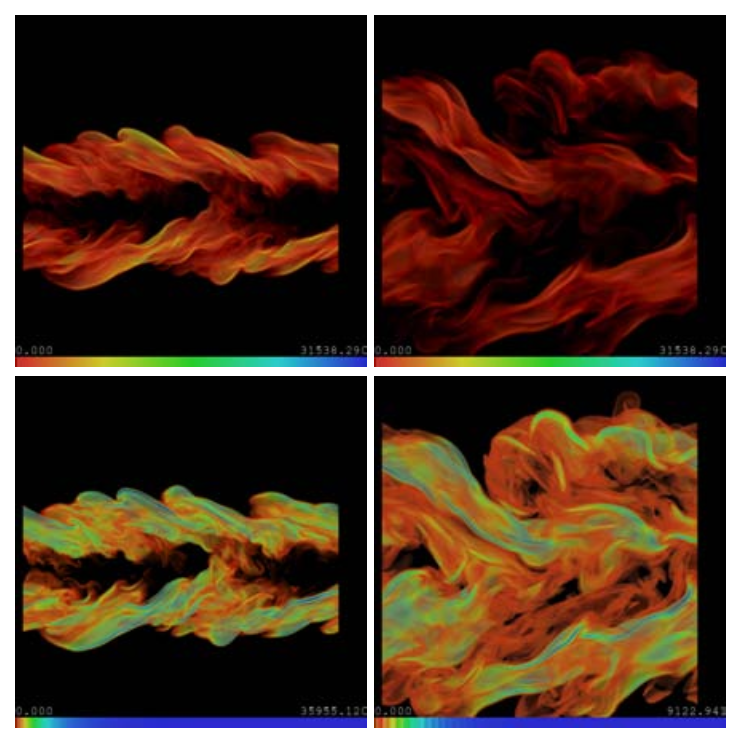
\includegraphics[width=1\linewidth]{images/woodring_semi-automatic_2009}
	\caption[A single static transfer function cannot capture dynamic features.]{A single static transfer function cannot capture dynamic features. In the two images at the top, the features appear to vanish over time. On the other hand, the features are visible over time if a dynamic transfer function is used (the two images at the bottom) \cite{woodring_semi-automatic_2009}.}
	\label{fig:woodring_semi-automatic_2009}
\end{figure}

Ward and Guo \cite{ward_visual_2011} presented a method for visualizing time-series data that reveals a wide variety of features in the data, by mapping short sub-sequences of the time-varying volume data into a high-dimensional shape space, and then performing a dimension reduction process to allow projection into screen space.

Gu and Wang \cite{gu_transgraph:_2011} proposed an approach to organize a time-varying data set into a hierarchical graph, which captures the transition relationships in the data set. This approach assists the user in comprehending the correspondence between volume regions over time and allows interaction of the graph through brushing and liking.

In order to create coherent and feature-prominent animations of time-varying volume data, Peng et al. \cite{peng_optimal_2011} described an optimal color mapping strategy, which uses a two-phase optimization method with bilateral filtering and energy minimization.

%-------------------------------------------------------------------------
%-------------------------------------------------------------------------

%\section{Conclusions}


%-------------------------------------------------------------------------
	
%\bibliographystyle{eg-alpha}
\bibliographystyle{eg-alpha-doi-gv2}
	
\bibliography{bibliography}
	
%-------------------------------------------------------------------------
	
\end{document}

